\section{Reading text from Loday-Richaud}
\begin{itemize}
  \item \textbf{The paper:}
    \cite{Loday1994}
    \begin{itemize}
      \item Stokes matrices are not all germs of isotropies, only the Sokes
        germs! see 4.3.13
      \item for \textbf{Sheaf $\to$ Matrix}
        \begin{thm}[II.2.1]
          The map
          \[
            h:\prod_{\alpha\in\A}\Sto_\alpha(A_0)\to H^1(S^1;\Lambda(A_0))
          \]
          is bijective and natural.
        \end{thm}
    \end{itemize}
  \item \textbf{The book:} \cite{Loday2014}
    \begin{itemize}
      \item multilevels, multisectors
    \end{itemize}
  \item others:
    \begin{itemize}
      \item \cite{LodayRichaud2004}
    \end{itemize}
\end{itemize}

$k -1 \to k$

\subsection{Determination $\tilde\theta$ of $\theta$}
\begin{center}
  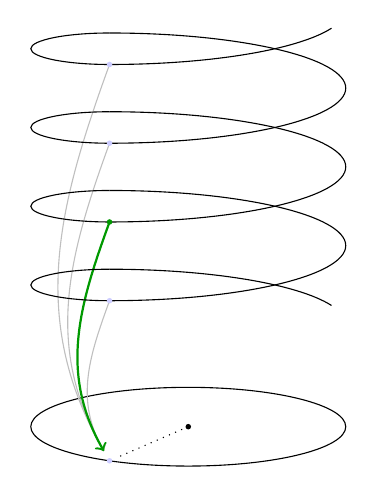
\begin{tikzpicture}[scale=1]
    \node[] (zero) at (0,0) {};
    \fill (zero) circle (1pt);
    \draw (0,-0.5) arc (270:-90:2 and 0.5);

    \node (theta) at ({cos(240) * 2},{sin(240) * 0.5}) {};
    % \node [below left of=theta,blue!40!white] {$\theta$};

    \draw[->,gray!50!white] (-1,1.6) to[out=250,in=120] (theta);
    \draw[->,gray!50!white] (-1,3.6) to[out=250,in=120] (theta);
    \draw[->,gray!50!white] (-1,4.6) to[out=250,in=120] (theta);
    \draw[->,green!60!black,thick] (-1,2.6) to[out=250,in=120] (theta);

    \draw[dotted] (0,0) -- (theta);
    \fill[blue!20!white] (theta) circle (1pt);


    \draw[] (-1,2) arc (270:200:-3 and -0.7);
    \draw[] (-1,2) arc (270:90:1 and -0.2) arc (270:90:-3 and 0.7);
    \fill[blue!20!white] (-1,1.6) circle (1pt);
    \draw[] (-1,3) arc (270:90:1 and -0.2) arc (270:90:-3 and 0.7);
    \fill[green!60!black] (-1,2.6) circle (1pt);
    \draw[] (-1,4) arc (270:90:1 and -0.2) arc (270:90:-3 and 0.7);
    \fill[blue!20!white] (-1,3.6) circle (1pt);
    \draw[] (-1,5) arc (270:90:1 and -0.2) arc (270:200:-3 and 0.7);
    \fill[blue!20!white] (-1,4.6) circle (1pt);
  \end{tikzpicture}
\end{center}

\subsection{Definition of $\Lambda_\theta(A_0)$}
$\Lambda_\theta(A_0)$ $:\Leftrightarrow{}$ sheaf of flat isotropies over $S^1$
\marginnote{p. 854f \cite{Loday1994}}
\begin{defn}
  A germ of $\Lambda_\theta(A_0)$ at $\theta_0\in S^1$ is
  \begin{itemize}
    \item an invertible Matrix $f\in\Gl_n(\cO(U))$
      \begin{itemize}
        \item for suitable arc $U=U(\theta_0,\epsilon,\epsilon')$
      \end{itemize}
      satisfying:
      \begin{enumerate}
        \item \emph{Flatness:}
          \[
            \underset{x\in U}{\underset{x\to0}{\lim}}f(x)=\Id
            \text{ and }
            f\underset{U}{\sim}I
          \]
        \item \emph{Isotropy of $[A_0]$: ${}^f\!A_0=A_0$.}
      \end{enumerate}
  \end{itemize}
\end{defn}

\begin{center}
  \begin{tikzpicture}[scale=1]
    \node[] (zero) at (0,0) {};
    \fill (zero) circle (1pt);

    \fill[blue!20!white] (theta) circle (1pt);

    \filldraw[fill=green!20!white
      ,draw=green!60!black
      ,thick
    ,path fading=west] (0,0)
      -- ({cos( -50 )*4},{sin( -50 )*1}) arc (-50:20:4 and 1)
      -- cycle;

    \filldraw[fill=green!20!white
      ,draw=green!60!black
      ,thick
    ,path fading=west] (0,4)
      -- ({cos( -50 )*0.5},{4 + sin( -50 )*2})
      -- ({cos( -50 )*0.5 + cos( -10 )*3}
        ,{4 + sin( -50 )*2 + sin( -10 )*12})
      arc (-80:40:1 and 3)
      -- ({cos( 20 )*0.5},{4 + sin( 20 )*2})
      -- cycle;

    \fill[fill=white,draw=black] (0,2) arc (270:-90:0.5 and 2);

    \draw[blue!60!black,path fading=east]
      (zero) -- ({cos( -15 )*4},{sin( -15 )*1});

    \draw[dashed] (zero) -- (0,2);
  \end{tikzpicture}
\end{center}

\subsection{Definition of $\Sto_\alpha(A_0)$}
\begin{itemize}
  \item p. 861 in the paper
  \item p. 78 in the book
\end{itemize}

\subsection{Definition of $\cF$}

\subsection{Adequate coverings}
\begin{center}
  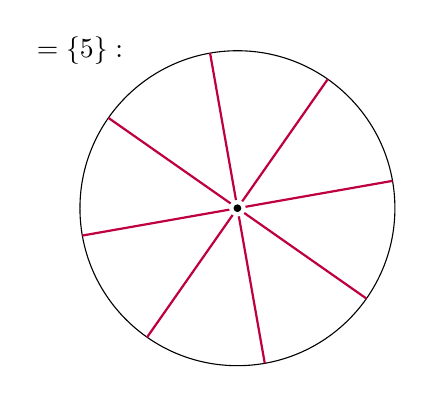
\begin{tikzpicture}[scale=2]
    \node (zero) at (0,0) {};
    \draw (zero) circle (1cm);

    \node at (-1,1) {$\cK=\{5\}:$};

    \foreach \w in {55}
    {\foreach \sep in {0,45,90,135,180,225,270,315}
     {\draw[thick,purple] (0,0) -- +({cos( \w + \sep )},{sin( \w + \sep )});}};

    \fill[white] (zero) circle (1.5pt);
    \fill (zero) circle (.7pt);
  \end{tikzpicture}
  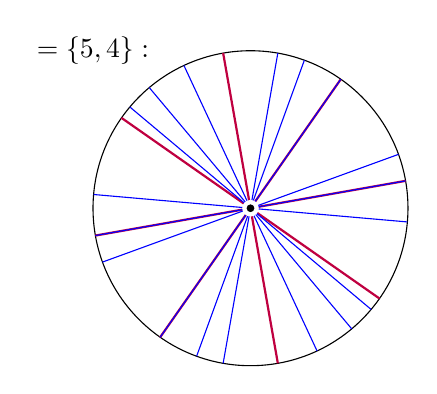
\begin{tikzpicture}[scale=2]
    \node (zero) at (0,0) {};
    \draw (zero) circle (1cm);

    \node at (-1,1) {$\cK=\{5,4\}:$};

    \foreach \w in {55}
    {\foreach \sep in {0,45,90,135,180,225,270,315}
     {\draw[thick,purple] (0,0) -- +({cos( \w + \sep )},{sin( \w + \sep )});}};

    \foreach \w in {10,20,55}
    {\foreach \sep in {0,60,120,180,240,300}
     {\draw[blue] (0,0) -- +({cos( \w + \sep )},{sin( \w + \sep )});}};

    \fill[white] (zero) circle (1.5pt);
    \fill (zero) circle (.7pt);
  \end{tikzpicture}
  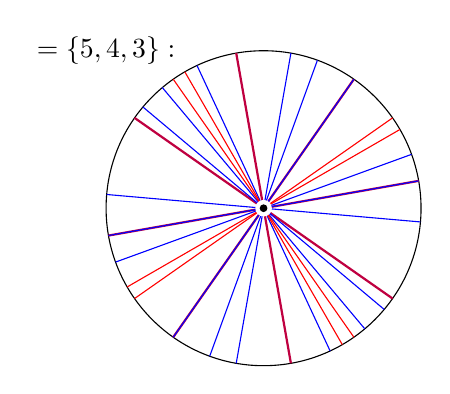
\begin{tikzpicture}[scale=2]
    \node (zero) at (0,0) {};
    \draw (zero) circle (1cm);

    \node at (-1,1) {$\cK=\{5,4,3\}:$};

    \foreach \w in {55}
    {\foreach \sep in {0,45,90,135,180,225,270,315}
     {\draw[thick,purple] (0,0) -- +({cos( \w + \sep )},{sin( \w + \sep )});}};

    \foreach \w in {10,20,55}
    {\foreach \sep in {0,60,120,180,240,300}
     {\draw[blue] (0,0) -- +({cos( \w + \sep )},{sin( \w + \sep )});}};

    \foreach \w in {30,35}
    {\foreach \sep in {0,90,180,270}
     {\draw[red] (0,0) -- +({cos( \w + \sep )},{sin( \w + \sep )});}};

    \fill[white] (zero) circle (1.5pt);
    \fill (zero) circle (.7pt);
  \end{tikzpicture}
\end{center}

Let $k\in\cK$.
\subsubsection{The \emph{cyclic covering $\cU^k=\{U_\alpha^k;\alpha\in\A^k\}$}}
\begin{center}
  \begin{tikzpicture}[scale=2.5]
    \node (zero) at (0,0) {};
    \draw (zero) circle (1cm);

    \node at (-1,1) {$\textcolor{purple}{\dot\cU^{5}}:$};
    \node at (-1.6,1.6) {$\textcolor{blue}{\dot\cU^{4}}:$};
    \node at (-2,2) {$\textcolor{green!60!black}{\dot\cU^{3}}:$};

    %%%%%%%%%%%%%%%%%%%%%%%%%%%%%%%%%%%%%%%%%%%%%%%%%%%%%%%%%%%%%%%%%%%%%%%%%%%
    %%%%  Purple
    \foreach \w in {10,25}
    {\foreach \sep in {0,45,90,135,180,225,270,315}
     {\draw[thick,purple] (0,0) -- +({cos( \w + \sep )},{sin( \w + \sep )});

      \pgfmathsetmacro\r{{1.1 + mod(\w,10)/100 + mod(\sep,2)/10}}
      \draw[dotted,purple] ({cos( \w + \sep )},{sin( \w + \sep )})
        -- ({cos( \w + \sep) * \r},{sin( \w + \sep) * \r});

      \draw[thick,purple] ({cos( \w + \sep -22) * \r},{sin( \w + \sep -22) * \r})
        arc ({\w + \sep - 22}:{\w + \sep +22}:\r);
      }};

    %%%%%%%%%%%%%%%%%%%%%%%%%%%%%%%%%%%%%%%%%%%%%%%%%%%%%%%%%%%%%%%%%%%%%%%%%%%
    %%%%  Blue
    \foreach \w in {10,20,55}
    {\foreach \sep in {0,60,120,180,240,300}
     {\draw[blue] (0,0) -- +({cos( \w + \sep ) * 0.9},{sin( \w + \sep ) * 0.9});}};

    \foreach \sep in {0,180}
    {\pgfmathsetmacro\rr{1.6}
     \foreach \w in {10,20,55
                    ,70,80,115
                    ,130,140,175}
     {\pgfmathsetmacro\rr{{\rr + (mod(\w,60) - 5*mod(\w,10))/150 
                               + mod(\w + \sep - mod(\w,60),120)/300}}
      \draw[dotted,blue] ({cos( \w + \sep )},{sin( \w + \sep )})
        -- ({cos( \w + \sep) * \rr},{sin( \w + \sep) * \rr});
      \draw[blue,thick] ({cos(\sep+\w -29) * \rr},{sin(\sep+\w -29) * \rr})
        arc ({\sep+\w -29}:{\sep+\w +29}:\rr);
     }
    }

    %%%%%%%%%%%%%%%%%%%%%%%%%%%%%%%%%%%%%%%%%%%%%%%%%%%%%%%%%%%%%%%%%%%%%%%%%%%
    %%%%  Green
    \foreach \w in {30,35}
    {\foreach \sep in {0,90,180,270}
     {\draw[green!60!black] (0,0) -- +({cos( \w + \sep ) * 0.8},{sin( \w + \sep) * 0.8});}};

    \foreach \sep in {0,180}
    {\pgfmathsetmacro\rr{2.4}
     \foreach \w in {30,35
                    ,120,125}
     {\pgfmathsetmacro\rr{{\rr + mod(\w,10)/100 + mod(\w-mod(\w,90),180)/900}}
      \draw[dotted,green!60!black] ({cos( \w + \sep )},{sin( \w + \sep )})
        -- ({cos( \w + \sep) * \rr},{sin( \w + \sep) * \rr});
      \draw[green!60!black,thick] ({cos(\sep+\w -44) * \rr},{sin(\sep+\w -44) * \rr})
        arc ({\sep+\w -44}:{\sep+\w +44}:\rr);
     }
    }

    \fill[white] (zero) circle (1.5pt);
    \fill (zero) circle (.7pt);
  \end{tikzpicture}
\end{center}

\subsubsection{The \emph{cyclic covering
  $\cU^{\leq k}=\{U_\alpha^{\leq k};\alpha\in\A^{\leq k}\}$}}
\begin{center}
  \begin{tikzpicture}[scale=2.5]
    \node (zero) at (0,0) {};
    \draw (zero) circle (1cm);

    \node at (-1.05,1.05) {$\textcolor{purple}{\dot\cU^{\leq 5}}:$};
    \node at (-1.65,1.65) {$\textcolor{blue}{\dot\cU^{\leq 4}}:$};
    \node at (-2.05,2.05) {$\textcolor{green!60!black}{\dot\cU^{\leq 3}}:$};

    %%%%%%%%%%%%%%%%%%%%%%%%%%%%%%%%%%%%%%%%%%%%%%%%%%%%%%%%%%%%%%%%%%%%%%%%%%%
    %%%%  Purple
    \foreach \w in {10,25}
    % {\foreach \sep in {0,45,90,135,180,225,270,315}
    {\foreach \sep in {0,36,72,108,144,180,216,252,288,324}
     {\draw[thick,purple] (0,0) -- +({cos( \w + \sep )},{sin( \w + \sep )});

      \pgfmathsetmacro\r{{1.1 + mod(\w,10)/100 + mod(\sep,72)/360}}
      \draw[dotted,purple] ({cos( \w + \sep )},{sin( \w + \sep )})
        -- ({cos( \w + \sep) * \r},{sin( \w + \sep) * \r});

      \draw[thick,purple] ({cos( \w + \sep -17.5) * \r},{sin( \w + \sep -17.5) * \r})
        arc ({\w + \sep - 17.5}:{\w + \sep +17.5}:\r);

      % \draw[purple] ({cos( \w + \sep -17.5) * \r},{sin( \w + \sep -17.5) * \r})
      %   -- ({cos( \w + \sep -17.5) * 1.5},{sin( \w + \sep -17.5) * 1.5});
      % \draw[purple] ({cos( \w + \sep +17.5) * \r},{sin( \w + \sep +17.5) * \r})
      %   -- ({cos( \w + \sep +17.5) * 1.5},{sin( \w + \sep +17.5) * 1.5});
      }};

    %%%%%%%%%%%%%%%%%%%%%%%%%%%%%%%%%%%%%%%%%%%%%%%%%%%%%%%%%%%%%%%%%%%%%%%%%%%
    %%%%  Blue
    \foreach \w in {10,20,55}
    {\foreach \sep in {0,60,120,180,240,300}
     {\draw[blue] (0,0) -- +({cos( \w + \sep ) * 0.9},{sin( \w + \sep ) * 0.9});}};

    \foreach \sep in {0,180}
    {\foreach \w in {10,20,55
                    ,70,80,115
                    ,130,140,175}
     {\pgfmathsetmacro\rr{{1.7 + (mod(\w,60) - 5*mod(\w,10))/150 
                               + mod(\w + \sep - mod(\w,60),120)/300}}
      \draw[dotted,blue] ({cos( \w + \sep )},{sin( \w + \sep )})
        -- ({cos( \w + \sep) * \rr},{sin( \w + \sep) * \rr});
      \draw[gray!42!white] ({cos(\sep+\w -29) * \rr},{sin(\sep+\w -29) * \rr})
        arc ({\sep+\w -29}:{\sep+\w +29}:\rr);

      % \draw[gray!42!white] ({cos( \w + \sep -29) * \rr},{sin( \w + \sep -29) * \rr})
      %   -- ({cos( \w + \sep -29) * 1.5},{sin( \w + \sep -29) * 1.5});
      % \draw[gray!42!white] ({cos( \w + \sep +29) * \rr},{sin( \w + \sep +29) * \rr})
      %   -- ({cos( \w + \sep +29) * 1.5},{sin( \w + \sep +29) * 1.5});
     }

     \pgfmathsetmacro\w{10}
     \pgfmathsetmacro\rr{{1.7 + (mod(\w,60) - 5*mod(\w,10))/150 
                              + mod(\w + \sep - mod(\w,60),120)/300}}
     \draw[thick,blue] ({cos(\sep+\w -17.5) * \rr},{sin(\sep+\w -17.5) * \rr})
       arc ({\sep+\w -17.5}:{\sep+\w +17.5}:\rr);

     \pgfmathsetmacro\w{20}
     \pgfmathsetmacro\rr{{1.7 + (mod(\w,60) - 5*mod(\w,10))/150 
                              + mod(\w + \sep - mod(\w,60),120)/300}}
     \draw[thick,blue] ({cos(\sep+ -7.5) * \rr},{sin(\sep+ -7.5) * \rr})
       arc ({\sep+ -7.5}:{\sep+ 42.5}:\rr);

     \pgfmathsetmacro\w{55}
     \pgfmathsetmacro\rr{{1.7 + (mod(\w,60) - 5*mod(\w,10))/150 
                              + mod(\w + \sep - mod(\w,60),120)/300}}
     \draw[thick,blue] ({cos(\sep+ 28.5) * \rr},{sin(\sep+ 28.5) * \rr})
       arc ({\sep+ 28.5}:{\sep+ 78.5}:\rr);

     \pgfmathsetmacro\w{70}
     \pgfmathsetmacro\rr{{1.7 + (mod(\w,60) - 5*mod(\w,10))/150 
                              + mod(\w + \sep - mod(\w,60),120)/300}}
     \draw[thick,blue] ({cos(\sep+ 43.5) * \rr},{sin(\sep+ 43.5) * \rr})
       arc ({\sep+ 43.5}:{\sep + \w + 29}:\rr);

     \pgfmathsetmacro\w{80}
     \pgfmathsetmacro\rr{{1.7 + (mod(\w,60) - 5*mod(\w,10))/150 
                              + mod(\w + \sep - mod(\w,60),120)/300}}
     \draw[thick,blue] ({cos(\sep+ \w - 29) * \rr},{sin(\sep+ \w - 29) * \rr})
       arc ({\sep+ \w - 29}:{\sep + 99.5}:\rr);

     \pgfmathsetmacro\w{115}
     \pgfmathsetmacro\rr{{1.7 + (mod(\w,60) - 5*mod(\w,10))/150 
                              + mod(\w + \sep - mod(\w,60),120)/300}}
     \draw[thick,blue] ({cos(\sep+ \w - 29) * \rr},{sin(\sep+ \w - 29) * \rr})
       arc ({\sep+ \w - 29}:{\sep + 135.5}:\rr);

     \pgfmathsetmacro\w{130}
     \pgfmathsetmacro\rr{{1.7 + (mod(\w,60) - 5*mod(\w,10))/150 
                              + mod(\w + \sep - mod(\w,60),120)/300}}
     \draw[thick,blue] ({cos(\sep+ \w - 29) * \rr},{sin(\sep+ \w - 29) * \rr})
       arc ({\sep+ \w - 29}:{\sep + 150.5}:\rr);

     \pgfmathsetmacro\w{140}
     \pgfmathsetmacro\rr{{1.7 + (mod(\w,60) - 5*mod(\w,10))/150 
                              + mod(\w + \sep - mod(\w,60),120)/300}}
     \draw[thick,blue] ({cos(\sep+ 115.5) * \rr},{sin(\sep+ 115.5) * \rr})
       arc ({\sep+ 115.5}:{\sep + \w + 29}:\rr);

     \pgfmathsetmacro\w{175}
     \pgfmathsetmacro\rr{{1.7 + (mod(\w,60) - 5*mod(\w,10))/150 
                              + mod(\w + \sep - mod(\w,60),120)/300}}
     \draw[thick,blue] ({cos(\sep+ 151.5) * \rr},{sin(\sep+ 151.5) * \rr})
       arc ({\sep+ 151.5}:{\sep + \w + 29}:\rr);
    }

    %%%%%%%%%%%%%%%%%%%%%%%%%%%%%%%%%%%%%%%%%%%%%%%%%%%%%%%%%%%%%%%%%%%%%%%%%%%
    %%%%  Green
    \foreach \w in {30,35}
    {\foreach \sep in {0,90,180,270}
     {\draw[green!60!black] (0,0) -- +({cos( \w + \sep ) * 0.8},{sin( \w + \sep) * 0.8});}};

    \foreach \sep in {0,180}
    {\foreach \w in {30,35
                    ,120,125}
     {\pgfmathsetmacro\rr{{2.5 + mod(\w,10)/100 + mod(\w-mod(\w,90),180)/900}}
      \draw[dotted,green!60!black] ({cos( \w + \sep )},{sin( \w + \sep )})
        -- ({cos( \w + \sep) * \rr},{sin( \w + \sep) * \rr});
      \draw[gray!42!white] ({cos(\sep+\w -44) * \rr},{sin(\sep+\w -44) * \rr})
        arc ({\sep+\w -44}:{\sep+\w +44}:\rr);
     }


     \pgfmathsetmacro\w{30}
     \pgfmathsetmacro\rr{{2.5 + mod(\w,10)/100 + mod(\w-mod(\w,90),180)/900}}
     \draw[thick,green!60!black] ({cos(\sep+ 7.5) * \rr},{sin(\sep+ 7.5) * \rr})
       arc ({\sep+ 7.5}:{\sep +63.5}:\rr);
     \pgfmathsetmacro\w{35}
     \pgfmathsetmacro\rr{{2.5 + mod(\w,10)/100 + mod(\w-mod(\w,90),180)/900}}
     \draw[thick,green!60!black] ({cos(\sep+ 7.5) * \rr},{sin(\sep+ 7.5) * \rr})
       arc ({\sep+ 7.5}:{\sep +63.5}:\rr);

     \pgfmathsetmacro\w{120}
     \pgfmathsetmacro\rr{{2.5 + mod(\w,10)/100 + mod(\w-mod(\w,90),180)/900}}
     \draw[thick,green!60!black] ({cos(\sep+ 100.5) * \rr},{sin(\sep+ 100.5) * \rr})
       arc ({\sep+ 100.5}:{\sep +150.5}:\rr);
     \pgfmathsetmacro\w{125}
     \pgfmathsetmacro\rr{{2.5 + mod(\w,10)/100 + mod(\w-mod(\w,90),180)/900}}
     \draw[thick,green!60!black] ({cos(\sep+ 100.5) * \rr},{sin(\sep+ 100.5) * \rr})
       arc ({\sep+ 100.5}:{\sep +150.5}:\rr);
    }

    \fill[white] (zero) circle (1.5pt);
    \fill (zero) circle (.7pt);
  \end{tikzpicture}
\end{center}

\subsection{Proof}
\subsubsection{Unique level} \marginnote{p. 872}
\subsubsection{Multi level} \marginnote{p. 872}
